\dateline{17 февраля 2018 г.}

\section*{Введение. Организационные моменты}

\textbf{\color{blue}! Лектор --- Степанов Евгений Олегович.}

\begin{quote}
  Вроде как считается, что на матмехе чуть больше уровень математической подготовки, и в этом должен быть ваш плюс.
\end{quote}

Курс в основном посвящен решению дифференциальных уравнений в частных производных и скорее всего так и должен называться --- <<Уравнения в частных производных>>. Текущее название --- <<Уравнения математической физики>> --- по большей части обусловлено историческими причинами.

Материал курса разбит на две главы --- первая посвящена классическим результатам математической физики, в то время как вторая является концептуально более свежей и посвящена обобщенным решениям (в основном --- решению задачи Дирихле для уравнения Пуассона и необходимым для этого средствам).

\subsection*{Устройство курса}

Обычный экзамен. Коллоквиума не будет; на 5 нужно сдать еще и задачу. Две (<<реально легкие>>) теоретические к/р, гарантирующие автомат (3 или 4) при нужном количестве баллов. Чтобы сдать на 5, нужно сдавать экзамен.

\subsection*{Необходимые знания}

\begin{itemize}
  \item Анализ вещественной переменной;
  \item Основные определения топологии;
  \item Мера Лебега и интеграл Лебега. Базовые определения:
    \begin{itemize}
      \item $\Omega \in \mathbb{R}^n$ --- область ($\equiv$ открытое множество),
      \item $L^1(\Omega)$ --- класс функций, измеримых по Лебегу,
      \item $L^p(\Omega) \coloneqq \{ u \colon \int_\Omega \abs{u(x)}^p \dd x < +\infty \}$,
      \item $L^\infty(\Omega) \coloneqq \{ u \colon \exists C > 0 \colon \abs{u(x)} \le c\ \text{почти всюду} \}$;
    \end{itemize}
  \item <<Неплохо бы уметь интегрировать по частям>>;
  \item <<Теорема Фубини и что-то еще примерно оттуда же>>;
  \item Умение работать с частными производными.
\end{itemize}

\clearpage

\section{Уравнения в частных производных}

В данной главе будут рассматриваться в основном классические результаты математической физики, многие которых получены еще в XIX веке и ранее.

\subsection{Транспортное уравнение и уравнение диффузии}

\subsubsection{Модель распространения загрязнения}

Прежде, чем говорить непосредственно о решении каких-либо уравнений, мы рассмотрим одну классическую модель. Пусть у нас имеется пятно воды в реке. Для простоты представим, что река у нас одномерная, а пятно представляет собой отрезок в $\mathbb{R}$. Будем считать, что река течет со скоростью $v$.

\begin{figure}[ht]
  \centering
  \includegraphics{1}
  \caption{Иллюстрация модели}
\end{figure}

Если мы возьмем отрезок $[x, x + \Delta x]$, то общая масса вещества, заключенного в нем, будет равна:
%
\begin{equation*}
  \int_x^{x + \Delta x} c(t, \xi) \dd \xi
\end{equation*}
где $c(t, x)$ --- концентрация вещества в точке $x$ в момент времени $t$.

Обозначим поток вещества, проходящего через точку $x$ \emph{направо}, через $q(t, x)$. Полагая, что $c(t, x)$ подчиняется закону сохранения массы (то есть, что все изменения массы приходят и уходят через границы отрезка), будем считать справедливым следующее:
%
\begin{equation*}
  \dv{t} \int_x^{x + \Delta x} c(t, \xi) \dd \xi = -q(t, x + \Delta x) + q(t, x)
\end{equation*}

Отсюда:
%
\begin{equation*}
  \frac{1}{\Delta x} \int_{x}^{x + \Delta x} \pdv{c}{t} (t, \xi) \dd \xi = \frac{q(t, x) - q(t, x + \Delta x)}{\Delta x}
\end{equation*}

Устремляя $\Delta x \to 0$ (мы можем сделать это в случае, если функции гладкие), получаем следующий закон:
%
\begin{equation*}
  \pdv{c}{t} (t, x) = - \pdv{q}{x} (t, x)
\end{equation*}

Вообще говоря, от чего у нас может зависеть поток через границы? Возможно три случая: либо происходит диффузия вещества в воде, либо снос вещества жидкостью, либо и то, и другое вместе.

\paragraph{Случай диффузии.}

В случае, когда мы имеем дело с диффузией, поток зависит от градиента концентрации: вещество за счет броуновского движения распространяется оттуда, где его больше, туда, где его меньше. Если записать это в в виде дифференциального закона, получим следующее:
%
\begin{equation*}
  q(t, x) = k \pdv{c}{x} (t, x)
\end{equation*}
%
где $k = -D$, $D > 0$ --- \emph{коэффициент диффузии (коэффициент Дарси)}.

Дифференцируя еще раз по $x$, получаем \emph{уравнение диффузии} (оно же \emph{уравнение теплопроводности}):
%
\begin{equation}
  \boxed{%
    \pdv{c}{t} (t, x) = D \pdv{c}{x}{x} (t, x)}
  \label{lecture1-diffusion}
\end{equation}

\paragraph{Случай конвекции.}

Возможен следующий случай: диффузии нет (чистый снос материала жидкостью). Тогда поток через границу очевидным образом зависит от скорости течения и концентрации вещества:
%
\begin{equation*}
  q(t, x) = vc(t, x)
\end{equation*}

Дифференцируя по $t$, получаем \emph{транспортное уравнение} (оно же \emph{закон сохранения массы при конвекции} или \emph{уравнение переноса}):
%
\begin{equation}
  \boxed{%
    \pdv{c}{t} (t, x) = - v \pdv{c}{x} (t, x)}
  \label{lecture1-transport}
\end{equation}
%
Это линейное уравнение 2-го порядка.

\paragraph{Общий случай.}

Возможен и третий случай (диффузия + конвекция). Тогда мы можем просто просуммировать факторы, влияющие на величину потока:
%
\begin{equation*}
  q(t, x) = -D \pdv{c}{x} (t, x) + v c(t, x)
\end{equation*}
%
Отсюда дифференцированием по $t$ можно вывести \emph{уравнение диффузии с конвективным членом}:
%
\begin{equation}
  \boxed{%
    \pdv{c}{t}(t, x) = D \pdv{c}{x}{x} (t, x) - v \pdv{c}{x} (t, x)}
  \label{lecture1-diffusion-transport}
\end{equation}

\subsubsection{Решение однородного транспортного уравнения}

Пусть нам требуется найти решения уравнения \eqref{lecture1-transport} с некоторыми начальными условиями. Поставим задачу Коши:
%
\begin{equation}
  \left\{\begin{aligned}
    &\pdv{c}{t} (t, x) + v \pdv{c}{x} (t, x) = 0 \\
    &c(0, x) = c_0(x)
  \end{aligned}\right.
  \label{lecture1-transport-cauchy}
\end{equation}

В данный момент нас интересует \emph{классическое решение} данной задачи, потому что никаких других решений мы пока не знаем. Классическое решение подразумевает, что функции должны быть достаточно гладкими, чтобы подстановка решения в уравнения была определена и мы получили тождество.

Если мы вернемся к модели, то можем увидеть, что каждая частица нашей массы эволюционирует следующим образом:
%
\begin{equation}
  \left\{\begin{aligned}
    \dv{x}{t} &= v \\
    \eval{x}_{t=0} &= x_0
  \end{aligned}\right.
  \label{lecture1-transport-particle}
\end{equation}

Есть догадка, что $c(t, x(t))$ --- константа. Докажем это аналитически. Продифференцируем концентрацию по $t$:
%
\begin{equation*}
  \dv{t} c(t, x(t)) = \pdv{c}{t} (t, x(t)) + \pdv{c}{x} (t, x(t)) \cdot \dv{x}{t}
\end{equation*}
%
Согласно \eqref{lecture1-transport-cauchy} и \eqref{lecture1-transport-particle}, правая часть равна $0$.

Исходя из нашей догадки и закона движения частиц массы, можем записать классическое решение:
%
\begin{equation}
  \boxed{%
    c(t, x) = c_0(x - vt)}
  \label{lecture1-travelling-wave}
\end{equation}

Можем проиллюстрировать решение следующим образом:

\begin{figure}[ht]
  \centering
  \includegraphics{2}
  \caption{Иллюстрация решения}
\end{figure}
%
Здесь показаны линии, соответствующие отдельно взятым частицам. Вдоль этих линий концентрация вещества остается постоянной --- то есть, с течением времени просто происходит снос вещества с постоянной скоростью

\begin{quote}
  Если кто-то во все-это не верит/не понял/не запомнил --- наплевать, берем формулу и подставляем.
\end{quote}

Получившийся результат можем оформить в виде теоремы:
%
\begin{thm}
  Если $c_0 \in C^1(\mathbb{R})$, то \eqref{lecture1-travelling-wave} --- это единственное решение\footnote{<<Под решением здесь все еще подразумевается классическое>>} задачи Коши \eqref{lecture1-transport-cauchy}.
\end{thm}

Такое решение называется решением бегущей волны (travelling wave)\footnote{Что прекрасно иллюстрируется картинкой :)}:
%
\begin{figure}[ht]
  \centering
  \includegraphics[scale=0.5]{3}
  \caption{Travelling wave}
\end{figure}

\subsubsection{Решение неоднородного транспортного уравнения}

Теперь предположим, что в правой части $\eqref{lecture1-transport-cauchy}$ у нас возникло какое-то возмущение, описываемое функцией $f(t, x)$. Рассмотрим теперь другую задачу:
%
\begin{equation}
  \left\{\begin{aligned}
    &\pdv{c}{t} + v \pdv{c}{x} = f(t, x) \\
    &c(0, x)) = c_0(x)
  \end{aligned}\right.
  \label{lecture1-transport-nonhom}
\end{equation}

Аналогично случаю однородного транспортного уравнения, рассмотрим производную по времени $c(t, x(t))$:
%
\begin{equation*}
  \dv{t} c(t, x(t)) = \pdv{c}{t} + \pdv{c}{x} \cdot \dv{x}{t} = \pdv{c}{t} + v \pdv{c}{x} = f(t, x(t))
\end{equation*}

В частности, если частицы движутся с постоянной скоростью, для любого $x_0$ мы имеем:
\begin{equation*}
  \dv{t} c(t, x_0 + vt) = f(t, x_0 + vt)
\end{equation*}
%
и можем проинтегрировать:
%
\begin{equation*}
  c(t, x_0 + vt) = c(0, x_0) + \int_0^t f(s, x_0 + vs) \dd s
\end{equation*}

Так как $x = x_0 + vt$, выразим $x_0 = x - vt$ и подставим:
%
\begin{equation*}
  \begin{aligned}
  c(t, x) &= c(0, x - vt) + \int_0^t f(s, x - vt + vs) \dd s\\
  &= c_0(x - vt) + \int_0^t f(s, x - v(t - s)) \dd s
  \end{aligned}
\end{equation*}

Теперь нам остается обеспечить лишь необходимую гладкость функций, чтобы полученная формула стала классическим решением задачи. Оформим получившийся результат в виде теоремы:
%
\begin{thm}
  Если $c_0 \in C^1(\mathbb{R})$, $f \in C(\mathbb{R}^+, \mathbb{R})$ и $\pdv{f}{x} \in C(\mathbb{R}^+, \mathbb{R})$, то
  %
  \begin{equation}
    \boxed{%
      c(t, x) = c_0(x - vt) + \int_0^t f(s, x - v(t - s)) \dd s}
    \label{lecture1-transport-nonhom-sol}
  \end{equation}
  %
  --- единственное (классическое) решение \eqref{lecture1-transport-nonhom}.
\end{thm}

\subsection{Основная лемма вариационного исчисления}

Полученный в данном параграфе результат потребуется нам в дальнейшем при решении волнового уравнения.

\subsubsection{Формулировки}

В вариационном исчислении центральное место занимает лемма Дюбуа-Реймона. Мы рассмотрим ее в двух формулировках и докажем более слабую из них.

\begin{lem}\emph{(лемма Дюбуа-Реймона, слабая формулировка)}
  $\Omega \in \mathbb{R}^n$ --- область, $f \in C(\Omega)$ и выполняется
  %
  \begin{equation}
    \int_\Omega f(x) g(x) \dd x = 0 \label{lecture1-dubois-condition}
  \end{equation}
  %
  для любых $g \in C_0^\infty(\Omega)$.\footnote{Напоминание: $\supp g \coloneqq \overline{\{x \colon g(x) \neq 0 \}}$ --- носитель функции, $C_0^k$ --- семейство функций с компактным носителем, у которых первые $k$ производных непрерывны.} Тогда $f \equiv 0$.
\end{lem}

\begin{lem}\emph{(лемма Дюбуа-Реймона, сильная формулировка)}
  $\Omega \in \mathbb{R}^n$ --- область, {\color{red} $f \in L^1_{\mathrm{loc}}(\Omega)$} и выполняется \eqref{lecture1-dubois-condition} для любых $g \in C_0^\infty(\Omega)$. Тогда $f \equiv 0$ {\color{red} почти всюду в $\Omega$}.
\end{lem}

\subsubsection{Доказательство леммы в слабой формулировке}

\begin{proof}
  От противного. Пусть $f \in C(\Omega)$ удовлетворяет \eqref{lecture1-dubois-condition} и $\exists x_0 \in \Omega$ такое, что $f(x_0) \neq 0$ (для определенности пусть $f(x_0) > 0$).
  
  В силу непрерывности $f$ существует $r > 0$ такое, что $f(x) > 0\ \forall x \in B_r(x_0) \subset \Omega$. Возьмем функцию $g(x) \in C^\infty(\Omega)$, которая бы всюду на $B_r(x_0)$ больше $0$, а всюду вне $B_r(x_0)$ --- равна $0$. Ясно, что $\supp g = \overline{B_r(x_0)} \Subset \Omega$,\footnote{$A \Subset B$ означает, что $A$ --- компактное подмножество $B$} тем самым $g \in C_0^\infty(\Omega)$.
  
  Мы знаем, что по условию:
  %
  \begin{equation*}
    \int_\Omega f(x) g(x) \dd x = 0
  \end{equation*}
  
  С другой стороны:
  %
  \begin{equation}
    \begin{aligned}
      \int_\Omega f(x) g(x) \dd x &= \int_{B_r(x_0)} f(x) g(x) \dd x + \int_{\Omega \setminus B_r(x_0)} f(x) g(x) \dd x \\
      &= \int_{B_r(x_0)} f(x) g(x) \dd x \\
      &> 0
    \end{aligned}
    \label{lecture1-estimation}
  \end{equation}
  %
  Последнее справедливо в силу того, что обе функции положительны на области ненулевой меры.
  
  Осталось доказать, что нужная функция $g$ существует. Определим $\psi \colon \mathbb{R} \to \mathbb{R}$:
  %
  \begin{equation*}
    \psi(x) \coloneqq \begin{cases}
      e^{1/\qty(x^2 - 1)} & x \in (-1, 1) \\
      0 & \text{иначе}
    \end{cases}
  \end{equation*}
  
  График такой функции выглядит следующим образом:
  %
  \begin{figure}[ht]
    \centering
    \includegraphics{4}
    \caption{График функции $\psi(x)$}
  \end{figure}

  Положим $g(x) \coloneqq \psi(\abs{x - x_0} / r)$ --- ни что иное, как тело вращения такой функции относительно оси, параллельной оси ординат и проходящей через точку $x_0$. Нетрудно показать, что она действительно удовлетворяет необходимым условиям.
  %
  \begin{figure}[ht]
    \centering
    \includegraphics{5}
    \caption{График функции $g(x)$ для двумерного случая}
  \end{figure}
  
  Таким образом, получаем, что \eqref{lecture1-estimation} противоречит \eqref{lecture1-dubois-condition}. Теорема доказана.
\end{proof}

\subsection{Колебания струны и волновое уравнение}

Рассмотрим еще одну модель. Теперь нам хотелось бы описать колебания струны уравнением.

\subsubsection{Модель и формулировка задачи}

Пусть у нас есть струна, выведенная из состояния равновесия. Струна определена на отрезке $[0, L]$ и описывается координатой $x$ и смещением отностительно состояния равновесия $u = u(t, x)$:
%
\begin{figure}[ht]
  \centering
  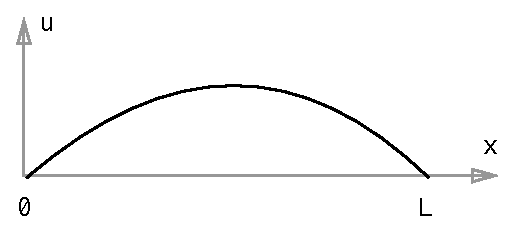
\includegraphics{6}
  \caption{Иллюстрация модели}
\end{figure}

Динамика такой системы подчиняется принципу, сформулированному в свое время еще Лагранжем --- \emph{принципу минимума действия}. Формулируется он следующим образом:
%
\begin{equation}
  A = \int_0^\tau (T - U) \dd t \longrightarrow \min
  \label{lecture1-lagrange}
\end{equation}
%
где $A$ --- работа, $T$ --- кинетическая энергия, $U$ --- потенциальная энергия.

Кинетическая энергия одного маленького отрезка струны равна:
%
\begin{equation*}
  \frac{u_t^2}{2} \rho_0 \Delta x
\end{equation*}

Кинетическая энергия всей струны находится как предел риманновой суммы при измельчении разбиения:
%
\begin{equation}
  T = \int_0^L \rho_0 \frac{u_t^2}{2} \dd x
  \label{lecture1-kinetic}
\end{equation}

Теперь нам необходимо найти потенциальную энергию, заключенную в кусочке струны $[x, x+\Delta x]$. Изначально ее длина была $\Delta x$, но после того, как она была выведена из состояния равновесия, ее длину можно выразить по формуле длины дуги $\int_x^{x + \Delta x} \sqrt{1 + u_x^2}\ \dd x$. Потенциальную энергию будем считать как разность:
%
\begin{equation}
  \begin{aligned}
    \int_x^{x + \Delta x} \sqrt{1 + u_x^2}\ \dd x - \Delta x &= \int_x^{x + \Delta x} \sqrt{1 + y_x^2 - 1}\ \dd x \\
    &\approx \int_x^{x + \Delta x} \left(1 + \frac{u_x^2}{2} - 1\right) \dd x \\
    &= \frac{1}{2} u_x^2 \Delta x
  \end{aligned}
  \label{lecture1-potential}
\end{equation}
%
где приближение обусловлено тем, что квадрат смещения струны пренебрежимо мал по отношению к ее длине.

Работу всей струны можем расписать как \eqref{lecture1-lagrange} с подстановкой \eqref{lecture1-kinetic} и \eqref{lecture1-potential}:
%
\begin{equation}
  \begin{aligned}
    A &= \int_0^\tau \dd t \left(\int_0^L \frac{\rho_0}{2} u_t^2 \dd x - \int_0^L \frac{\tau_0}{2} u_x^2 \dd x \right) \\
    &= \frac{1}{2} \int_0^\tau \dd t \int_0^L \dd x \left(\rho_0 u_t^2 - \tau_0 u_x^2 \right)
  \end{aligned}
  \label{lecture1-wave-functional}
\end{equation}